\documentclass[12pt]{article}
\usepackage[utf8]{inputenc}
\usepackage[top=0.75in, bottom=0.75in, left=0.75in, right=0.75in, headheight=15pt]{geometry}
\usepackage{amsmath, amssymb, amsthm, graphicx, hyperref, enumerate, multirow,  multicol, tikz, centernot, cancel, forest, lipsum, mathtools, bm, esvect, fancyhdr, esdiff, float, parskip, comment}

\DeclareMathSymbol{*}{\mathbin}{symbols}{"01} % change * to /cdot inside math
% \begingroup % let only this align, etc. break across pages
% \allowdisplaybreaks
% \begin{align}
%     ....
% \end{align}
% \endgroup

% \texorpdfstring{$k$}{k} math inside (sub/)section label

\pagestyle{fancy}
\fancyhead[L]{Liheng Cao}
% \fancyhead[C]{center}
\fancyhead[R]{}

\title{ML Homework 4}
\author{Liheng Cao}
% \date{Date}

\begin{document}
\maketitle

\section{}
When $ w_0 $ increases, then the probability of predicting class 1 becomes higher, and vice versa. 
\[ h(x) = \dfrac{1}{1+e^{-(w_0 + \cdots)}} \]
This is because as $ w_0 $ gets bigger, the result of exponentiation gets smaller. As the denominator gets smaller, the quotient gets larger. $ h(x) $ is used as the probability we will predict a certain class. The higher $ h(x) $ is, the more likely we will predict class 1 (as opposed to class 0).
\newpage

\section{}
The logistic function is \[ \dfrac{1}{1+e^{-\textbf{w}^T \textbf{x}}} \]
If we were to double $ \textbf{w} $, the result wouldn't actually change, as long as the threshold is 0.5. 

The geometric interpretation is because $ \textbf{w}^T\textbf{x} $ represents a (hyper)plane. Multiplying the equation of a plane doesn't affect any points that are on the plane (threshold = 0.5 $\implies$ on hyperplane), but it makes the points that are off it seem further away, increasing the certainty with which we pick a class. For example, if $ \textbf{w}^T\textbf{x} = 0$, then there is no change ($ 0 * 2 = 0 $). But if it's positive, it becomes a larger positive number, and vice versa.
\newpage

\section{}
\begin{enumerate}[(a)]
	\item 
	\[\begin{bmatrix}
		3 & 1 \\
		1 & 3 \\
	\end{bmatrix}\]
	
	\item :	
	\begin{figure}[H]
	    \centering
	    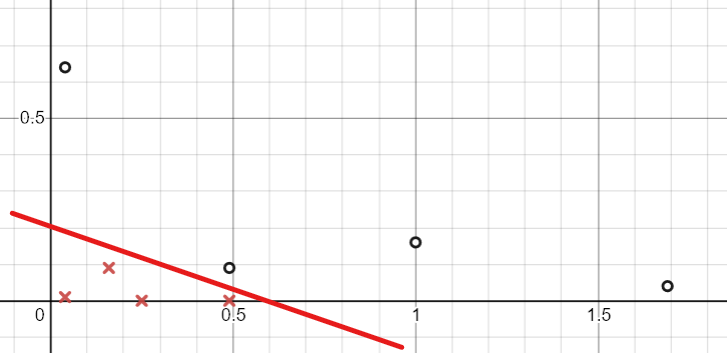
\includegraphics{images/3b.png}
	    \caption{o: class 0, x: class 1}
	    \label{fig:3:b}
	\end{figure}

	\item TPR = $ \dfrac{1}{3+1} = 1/4 $
	
	\item FPR = $ \dfrac{3}{3+1} = 3/4 $
	
	\item accuracy = $ \dfrac{3+3}{3 + 1 + 3 + 1} = 3/4 $
	
	\item recall = $ \dfrac{3}{3+1} = 3/4 $
	
	\item precision = $ \dfrac{3}{3+1} = 3/4 $
	
	\item \[ -[0 * \ln{(0.389)} + (1-0)\ln{(1-0.389)}] - \cdots - [1 * \ln{(0.638)} + (1-1)\ln{(1-0.638)}] = 4.25205106\ldots \]
	
	\item \[-\left[0*\ln{(\dfrac{1}{1+\exp{(-\mathbf{w'}^T\mathbf{X^{(1)}})}})}\right] + \cdots - \left[0*\ln{(\dfrac{1}{1+\exp{(-\mathbf{w'}^T\mathbf{X^{(8)}})}})}\right] = 3.0158793\ldots \]
	Since $\mathbf{w'}$ has a lower cross-entropy, it is a better fit for this data.
	
	\item 
	After one interation, \[ \mathbf{w} = \textbf{w} + \dfrac{\alpha}{N}\mathbf{x}^T \left(y - \sigma{(\textbf{x}\textbf{w})}\right) \]
	\[\begin{bmatrix}
		0.66\\
		-2.24\\
		-0.18\\
	\end{bmatrix}
	\]
	\[
	+
	\dfrac{0.1}{N} 
	\begin{bmatrix}
		1 & 1 & 1 & 1 & 1 & 1 & 1 & 1\\
		0.49 & 1.69 & 0.04 & 1 & 0.16 & 0.25 & 0.49 & 0.04\\
		0.09 & 0.04 & 0.64 & 0.16 & 0.09 & 0 & 0 & 0.01\\
	\end{bmatrix}
	\left(\begin{bmatrix}
		0\\
		0\\
		0\\
		0\\
		1\\
		1\\
		1\\
		1\\
	\end{bmatrix} - 
	\sigma \left(\begin{bmatrix}
	1 & 0.49 & 0.09\\
	1 & 1.69 & 0.04\\
	1 & 0.04 & 0.64\\
	1 & 1 & 0.16\\
	1 & 0.16 & 0.09\\
	1 & 0.25 & 0\\
	1 & 0.49 & 0\\
	1 & 0.04 & 0.01
	\end{bmatrix}
	\begin{bmatrix}
		0.66\\
		-2.24\\
		-0.18\\
	\end{bmatrix}
	\right)
	\right)
	\]
	\[=\begin{bmatrix}
		0.6683067\ldots\\
		-2.2394066\ldots\\
		-0.18515844\ldots\\
	\end{bmatrix}\]

	\item These data points would contribute a medium amount to the new \textbf{w}.
	
	\item These data points would contribute a low amount to the new \textbf{w}.
	
	\item These data points would contribute a high amount to the new \textbf{w}.
	
	\item \[-\left[0*\ln{(\dfrac{1}{1+\exp{(-\mathbf{w_g}^T\mathbf{X^{(1)}})}})}\right] + \cdots - \left[0*\ln{(\dfrac{1}{1+\exp{(-\mathbf{w_g}^T\mathbf{X^{(8)}})}})}\right] = 4.2519\ldots\]
	This is a very minor decrease from $ 4.2520 $. This makes sense because gradient ascent is supposed to make the model fit better and have less error.
\end{enumerate}
\newpage

\section{}
\begin{itemize}
	\item lasso \[ -\lambda\left(|w_1| + \cdots + |w_d|\right) + \sum\limits_{i=1}^{N} y^{(i)} \ln{(h(x))} + (1-y^{(i)})\ln{(1-h(x))} \]
	
	\item ridge \[ -\lambda\left(w_1^2 + \cdots + w_d^2\right) + \sum\limits_{i=1}^{N} y^{(i)} \ln{(h(x))} + (1-y^{(i)})\ln{(1-h(x))} \]
	
	\item gradient \[\textbf{x}^T(y-\sigma{(\textbf{x}\mathbf{w})}) - 2 \lambda I' \mathbf{w}\]
	
	\item Optimal $ \lambda = 0.6 $. It did help, or else the best lambda would be 0. The training error would get worse (no more overfitting), but the test/validation data would get better.
	\begin{figure}[H]
		\centering
		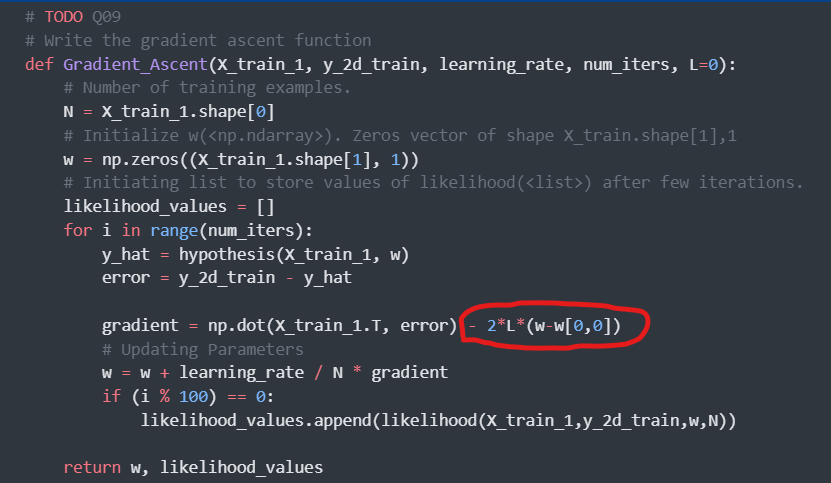
\includegraphics{images/ridgereg.png}
		\caption{Adding Ridge regression}
		\label{fig:4:ridgereg}
	\end{figure}
	
	\begin{figure}[H]
		\centering
		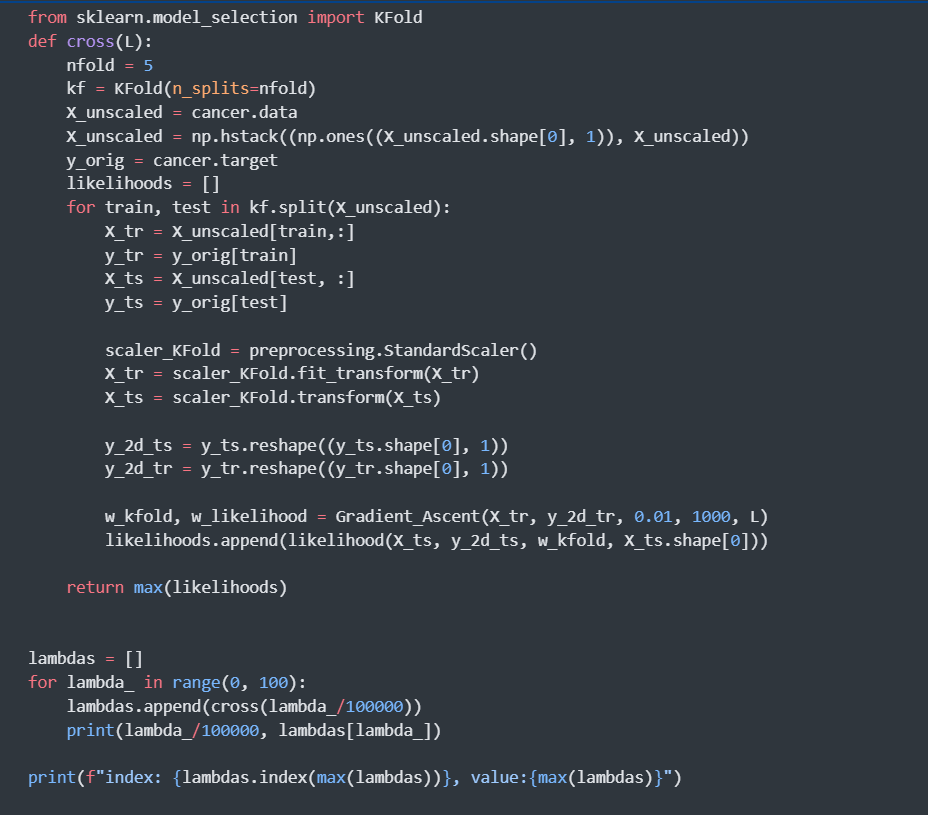
\includegraphics[width=\textwidth]{images/kfold.png}
		\caption{5 fold}
		\label{fig:4:kfold}
	\end{figure}	
\end{itemize}
Basically the code iterates over a range of lambdas and does cross validation on each, and then we see which one has the best errors.

Interestingly, if the iterations for gradient ascent were too low, I would actually get $ \lambda = 0 $ as the best error. I got $ \lambda = 0.6 $ from increasing the iterations and letting the code run for like 30 minutes. 
\newpage

\section{}
\begin{enumerate}[(a)]
	\item Predictors: average pitch; response: gender
	
	\item Predictors: matrix of where the strokes were; response: letter or number written
\end{enumerate}
\newpage

\section{}
\begin{enumerate}[(a)]
	\item 
	\begin{figure}[H]
		\centering
		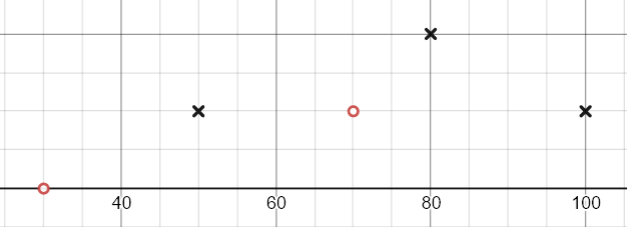
\includegraphics{images/6a.png}
		\caption{o: no donation, x: donation}
		\label{figure:6b}
	\end{figure}

	\item I will choose the horizontal line $ x_2 = 0.5 \implies 0.5 +0 * x_1 + w_2$
	\[ \mathbf{w}^T = [-0.5, 0, 1] \]
	
	\item The least likely would be the one that is incorrect. In this case, it's same 3, or the one that earns 70k, follows 1 site, and did not donate. No calculator was needed for this!
	
	\item They would not change the values of $ \hat{y} $, but they would change the likelihoods. If the prediction was correct, then the likelihood would increase. If the predictions were incorrect, then the likelihood would decrease.
\end{enumerate}



\end{document}